\documentclass{article}
\usepackage[utf8]{inputenc}
\usepackage[a4paper, includeheadfoot, margin=2.54cm]{geometry}

\usepackage{amsmath, amsthm, amssymb}
\newtheorem{definition}{Definition}
\newtheorem{theorem}{Theorem}

\usepackage[style=numeric]{biblatex}
\usepackage{graphicx}
\addbibresource{references.bib}

\title{History Independent Dynamic Partitioning}
\author{Shaya Rezai Yazdi \and Arvid Persson}

\begin{document}

\maketitle

\section{History independence}

\begin{definition}
    A data structure is said to be \textbf{history independent} (HI) if, given its internal representation, no information can be gained except the elements currently present in the data structure.
\end{definition}

\begin{definition}
    A data structure is \textbf{weakly history independent} (WHI) if the HI property holds on one inspection of the internal representation.
\end{definition}

\begin{definition}
    A data structure is \textbf{strongly history independent} (SHI) if the HI property holds on one inspection of the internal representation.
\end{definition}

\begin{definition}
    A data structure is \textbf{auditable} if it can easily be made HI on demand.
\end{definition}

The above definitions make two assumptions: observation takes place \textit{between} operations, never \textit{during} one; and any random state is initialized once such that all future operations are deterministic.

History independence is primarily a security or privacy feature. One might want to ensure that ``deleting'' some data actually wipes that data from memory and does not leave any trace of it ever having been there. This could prevent a password from leaking or certain attacks exploiting timing properties or heap fragmentation. Another example is in electronic voting systems where HI data structures could ensure that although an actor knows who has voted and even in what order they voted, they cannot determine anything about who voted for what.

\begin{theorem} \label{SHIcanon}
    A data structure is SHI if and only if it has a canonical representation.
\end{theorem}

\begin{proof}
    See \cite{SHIcanon}.
\end{proof}

This theorem has some useful consequences: two instances of a SHI data structure will be identical in memory (barring implementation detials), so equation and hashing is trivial. We also guarantee full reproducability, useful for formal verification and scientific computation.

Many common data structures are not HI. Consider for example the traditional binary search tree: the tree with 1 as its root and 2 as its right child is valid, but so is the tree with 2 as its root and 1 as its left child. Many variants such as AVL trees and red-black trees also fail. However, HI variants of binary search trees do exist, along with hash tables (using cuckoo hashing or linear probing), priority queues, memory allocators and more~\cite{HIDP}. By Theorem~\ref{SHIcanon}, we also observe that treaps, skiplists and many more data structures can easily be made SHI by using seeded randomness and a HI memory allocator.

\section{Dynamic partitioning}

\begin{definition}
    A collection of sets $G_i, 1 \le i \le k$ form \textbf{ordered groups} if $\forall 1 \le i \ne j \le k: (\forall x \in G_i, y \in G_j: x < y) \lor (\forall x \in G_i, y \in G_j: x > y)$. That is, all elements of any one set are smaller than all elements of any other set, or vice versa.
\end{definition}

The goal of a partitioning is to partition elements into ordered groups, each of size $\Theta(B)$ for some constant $B$. To make it dynamic, we also want to support insertions and deletions. For this purpose, we are interested in deterministic bounds~\cite{HIDP}.

\subsection{Dynamic partitioning in B-trees}

B-trees are a form of balanced search trees optimized for storage in external memory. They are integral to many databases and filesystems (e.g. NTFS, ext4). Each node contains between $\lceil \frac{m}{2} \rceil$ and $m$ children, except the root which is either a leaf or has at least two children. All leaves are on the same level. The value of $m$ is typically chosen to fill one disk block~\cite{Btree}.

B-trees support searches, insertions and deletions in $O(\log_m n)$ comparions and IO operations. Often useful are also range queries---finding all keys in a specified range.

\begin{definition}
    An event $e$ dependent on some number $n$ is said to occur \textbf{with high probability} (WHP) in $n$ if $\lim_{n \to \infty} \Pr\left[ e(n) \right] = 1$.
\end{definition}

B-tree balancing is entirely defined by maintaining a dynamic partitioning at each level of the tree. As a result of this, a traditonal B-tree is not HI. Some HI alternatives have been explored:

\begin{itemize}
    \item A B-skip-list~\cite{Bskip} is a skip list with the promotion probability modified from $\frac{1}{2}$ to $\frac{1}{m}$. There will be an expected $O(\log_m n)$ lists WHP and $m$ elements between non-promoted elements. However, the bounds are not deterministic and furthermore weak: elements with search cost $O(\log_2 n)$ exist WHP.

    \begin{itemize}
	\item With the restriction $m = O(\log^k n)$ and promotion probability $\frac{1}{\sqrt{m}}$, a search cost $O(\log_m n)$ is achieved WHP, but each block is only expected to be $\frac{1}{\sqrt{m}}$ full, leading to inefficient space usage and consequently degraded range query performance~\cite{Bskiprest}.
    \end{itemize}

    \item A treap can be modified to work with external memory, but offers weaker bounds for range queries and less efficient memory usage~\cite{Bskip}.

    \item A B-tree built on a packed-memory array achieves deterministic bounds, but lags behind in sequentiel insert performance and performs worse for some relationships of $m$ and $n$~\cite{Bskiprest}.
\end{itemize}

\section{History independent dynamic partitioning}

\subsection{Static $B/\alpha$ partitioning}

The paper starts by defining a static partitioning algorithm $B/\alpha$ partitioning to sort a sorted set $S$ into groups of sizes between $B/\alpha$ and $B$ where $B$ is the maximum group size and $\alpha$ is the tightness of the group. The general ``strategy'' (``Protect the flanks'', as referred to by the paper \cite{HIDP}) can be divided into three main steps:
\begin{enumerate}
    \item Divide the left/right-most endpoints of the sorted list $S$ into protected groups of size $(B/\alpha)$.
    \item Using a hash function, compute the minimum hash of the values in the unprotected middle region.
    \item Pivot the min(hash) value and recurse until the resulting endpoints are no larger than $B$.
\end{enumerate}

\begin{figure}
    \centering
    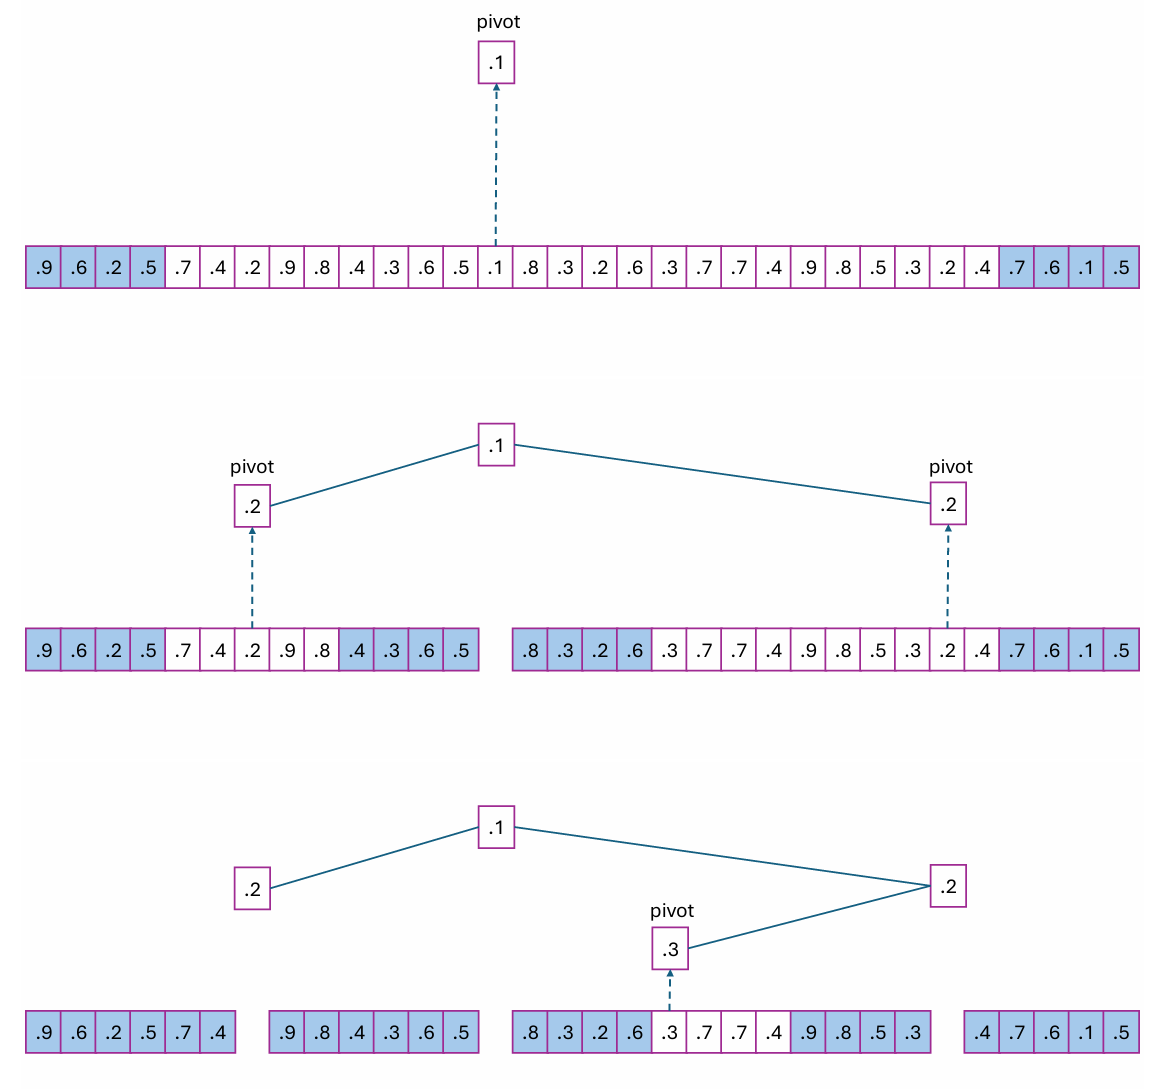
\includegraphics[width=0.5\linewidth]{images/pct.png}
    \caption{``Protect the flanks'' as shown by the paper where $B = 8$ and $\alpha = 2$. \cite{HIDP}}
    \label{fig:pct}
\end{figure}

\subsection{Protected Cartesian Tree (PCT) representation}

To allow for insertions/deletions whilst keeping the structure canonical the structure is represented as a \emph{Cartesian Tree}. This works exceptionally well due to the properties of a cartesian tree since they are built from an inorder sequence of values by rank along with a priority for every element (interpreted into the hash values of the static partition). \emph{Protected cartesian trees} is a term coined by the paper which enforces the protected group sizes $B/\alpha$ and stops the algorithm from picking a pivot from these groups.

\subsection{Measured Expected Costs}

The paper uses \emph{element-movement cost} and \emph{group-update cost} to show the cost of moving and reconstructing the tree.
\begin{definition}
    The \textbf{element-movement cost} of a dynamic partitioning is the number of elements that move from one group to another as part of an insertion or deletion, amortized. The theoretically optimal element-movement cost is $O(1)$~\cite{HIDP}.
\end{definition}

\begin{definition}
    The \textbf{group-update cost} of a dynamic partitioning is the number of group boundaries that move as part of an insertion or deletion, amortized. The theoretically optimal group-update cost is $O(\frac{1}{B})$~\cite{HIDP}.
\end{definition}

A practical HI B-tree should make it difficult or ideally infeasible to insert an element to trigger an expensive split, then remove that element to trigger an expensive merge, and repeat. The typical approach to preventing this kind of attack is to overallocate, creating new capacity only the first time that element is inserted and keeping it for later usage even if the element is deleted. This, however, could not possibly be HI. In the PCT representation, for an insertion/deletion to cause a larger split, the inserted/deleted value has to coincidentally be the pivot. The randomized hash function will, however, be effective at combating adversarial operations since the user wouldn't know their inputs hash value making the probability of a split $(\frac{1}{B})$.

\section{History independent B-tree}

Although we now have a HI Dynamic Partition, we would like to apply this to more commonly used data structures, namely a B-Tree. The way the paper constructs HI B-trees is by building it from the leaf level $T_{S0}$ and up.
\begin{enumerate}
    \item Start by applying the ``Protect the Flank'' strategy to the sorted set $S_0$ as normal where the protected groups become leaf nodes. The pivots are determined using \textbf{independent} hash functions $h_i$.
    \item The pivots become part of the next set $S_1$ where we apply the same strategy to the next level $T_{S1}$
    \item Repeat until the last pivot set $S_i$ is smaller or equal to the max group size $B$.
\end{enumerate}

\subsection{Insertions}

When a key is inserted into the HI B-tree;
\begin{itemize}
    \item The key is inserted into the correct position at the leaf level.
    \item If the leaf nodes size becomes larger than $B$ elements, the boundaries get re-calculated canonically using the hash independent hash function $h_0$.
    \item In case pivots get changed, the changes will continue upwards in the tree.
\end{itemize}

\subsection{Deletions}

Deletions work similarly but inversed;
\begin{itemize}
    \item When a key is removed and the node size becomes smaller than $B/\alpha$, the pivots get re-calculated and new groups are determined canonically because of the pivot selection rules.
    \item If a deleted key was a pivot, we promote the next smallest hash from the same unprotected region.
\end{itemize}

\subsection{HI B-tree Complexity}

The cost of insertions and deletions in HI B-trees can be divided into two types: 
\emph{expected cost}, and \emph{high probability cost}, which bounds the cost in most cases except extremely rare events.

\begin{table}[h]
    \centering
    \begin{tabular}{lcc}
	\hline
        \textbf{Cost Type}     & \textbf{Expected}                  & \textbf{With high probability}               \\ \hline
	Search cost (I/O)      & $O(\log_B n)$                      & $O(\log_B n)$                                \\
	Update cost (I/O)      & $O\left(\frac{\log_B n}{B}\right)$ & $O\left(\frac{\log n}{\log \log B}\right)$   \\
	Element movement       & $O(1)$                             & $O\left(B \frac{\log n}{\log \log n}\right)$ \\
	Group boundary updates & $O\left(\frac{1}{B}\right)$        & $O\left(\frac{\log n}{\log \log n}\right)$   \\ \hline
    \end{tabular}
    \caption{Expected and high probability costs in HI B-trees.}
\end{table}

\printbibliography

\end{document}
